% !TEX root = ../Thesis.tex

\chapter{Introduzione}
I satelliti SAR sono satelliti dotati di un radar ad apertura sintetica che permette
loro di acquisire immagini della superficie terrestre indipendentemente dalle 
condizioni meteorologiche e dalla luce solare. 
Missioni e piattaforme di riferimento includono Sentinel-1 (ESA) \cite{esa_sentinel1}, TerraSAR-X (DLR), 
COSMO-SkyMed (ASI) e RADARSAT.
I satelliti SAR, grazie a questa loro 
capacita, trovano applicazione in molteplici contesti. In ambito geologico \cite{nhess-20-2379-2020}, 
sono impiegati per il monitoraggio del suolo e dei processi 
geomorfologici, consentendo la mappatura di foreste, deserti e aree soggette a 
trasformazioni ambientali. Inoltre, risultano particolarmente efficaci nell’analisi 
dei fenomeni di deforestazione attraverso il rilevamento dei cambiamenti nella 
copertura boschiva. Marittimo, permettono di localizzare navi anche in condizioni 
meteorologiche avverse e di rilevare sversamenti di petrolio o altre sostanze 
inquinanti. Infrastrutture e urbanistica, vengono utilizzati per misurare gli 
spostamenti del terreno e delle aree urbane, oltre che per il controllo di dighe, 
ponti e ferrovie, e per l’osservazione dello sviluppo delle città. Il funzionamento 
di questo tipo di satellite come spiagato nel sito della \textit{N.A.S.A.} \cite{nasa_sar} si basa sull'uso di  onde radar che vengono inviate verso la Terra. 
Questi impulsi elettromagnetici rimbalzano sul terreno e sugli 
oggetti come edifici o vegetazione e tornano al satellite. 
Quest'ultimo analizzando il segnale di 
ritorno riesce ad ottenere informazioni sia sull'intensità del riflesso sia sul tempo impiegato 
dal segnale per tornare, dati fondamentali per ricostruire l'immagine del territorio. Il punto 
di forza del SAR è l'apertura sintetica. Poichè il satellite si muove lungo la sua orbita, i 
segnali raccolti in posizioni diverse vengono combinati insieme. Questo processo permette di 
simulare un'antenna molto più grande di quella reale, ottenendo così immagini ad altissima 
risoluzione, molto piu dettagliate di quelle che un radar di dimensioni fisiche limitate potrebbe 
generare da solo. In pratica, il movimento del satellite trasforma un radar relativamente piccolo 
in uno strumento potentissimo per osservare il pianeta. 
A seguito della cattura della scena di interesse, l’immagine ottenuta risulta disallineata, 
in quanto si genera un angolo $\theta$ tra l’asse del satellite e la superficie terrestre. 
Per correggere questo effetto, si applica una tecnica di allineamento dell’immagine \cite{HUGHES2020166}.
L'immagine generata dal satellite però presenta un particolare tipo di rumore. Quest'ultimo si forma quando un impulso radar colpisce il terreno, 
questo non riflette semplicemente un segnale uniforme. In realtà, il segnale viene riflesso da 
moltissimi piccoli scatter presenti sulla superficie come foglie, rocce o edifici. 
\begin{figure}[H]
    \centering
    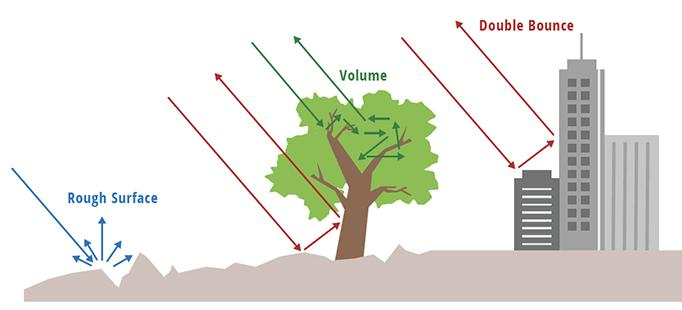
\includegraphics[width=0.8\textwidth]{utils/SARPolarization.jpg}
    \caption{Impulsi radar inviati dal satellite SAR verso la Terra e riflessi indietro.}
    \label{fig:sar_scatter}
\end{figure}
Tutti questi ritorni interferiscono tra di loro, sommando le onde con fasi diverse. Il risultato di questa 
interferenza prende il nome di Speckle. Questo tipo di rumore non è un errore del satellite o 
del radar, ma una caratteristica intrinseca del tipo di misura e si presenta con un pattern granuloso
che rende l'immagine difficile da interpretare ed analizzare.
Il processo di riduzione dello speckle 
prende il nome di despeckling \cite{1097762}. Quest'ultimo cerca di smussare o filtrare il rumore granulare senza 
però perdere le informazioni reali presenti nell'immagine. In letteratura vi sono molteplici 
approcci: alcui si basano su filtri spaziali che analizzano i pixel vicini, altri usano tecniche 
più sofisticate come metodi di deep learning. Ogni approccio ha i suoi
punti di forza e le sue lacune sulla base del tipo di ambiente rappresentato nell'immagine. 
Lo scopo di questa tesi è cercare di unire i punti di forza di alcuni modelli in modo da ottenere l’immagine
con il despeckling più accurato possibile. Un primo approccio per ottenere ciò consiste nell' utlizzare tecniche di machine learning
per predire la qualità di un immagine denoised attraverso una mappa di qualità. Ad ogni modello,
è associata una mappa che indica, pixel per pixel dove il modello ha funzionato meglio e 
dove invece peggio. La fusione avviene tramite la media pesata dove i relativi pesi 
sono le mappe di qualità. Questo approccio però non sfrutta al massimo i punti di forza 
di ogni singola immagine despeckled portando ad un risulato finale non soddisfacente, 
in quanto la qualità del denoising viene stimata concentrandosi sul singolo pixel senza 
guardare i vicini. Un secondo approccio più efficiente è basato sull’attenzione. Invece 
di utilizzare mappe di qualità che determinano la bontà del denoising di un singolo 
pixel, si utilizzano meccanismi basati sulla self e cross attention. Questo consente di andare oltre 
la valutazione locale pixel per pixel, mettendo in relazione l’informazione proveniente 
da più immagini despeckled e valorizzando i dettagli complementari.
La cross attention, infatti, nasce nel contesto della fusione multimodale di immagini 
(ad esempio infrarosso e visibile) e mira a combinare i punti di forza di diverse fonti 
mantenendo l’informazione complementare ed eliminando quella ridondante.
La chiave è che, mentre la self-attention tende a enfatizzare le correlazioni interne ad 
una singola immagine (quindi rischia di rafforzare il rumore residuo), la cross-attention 
sfrutta l’eterogeneità tra le diverse versioni despeckled per mettere in evidenza le 
informazioni non correlate, cioè i dettagli che risultano più affidabili in una ricostruzione 
ma assenti o degradati nelle altre. In questo modo il modello riesce a potenziare le componenti 
salienti e a ridurre le parti rumorose. Questo approccio consente di ottenere un’immagine despeckled più accurata e leggibile, perché 
tiene conto non solo del valore di ogni singolo pixel, ma anche del contesto e della complementarità 
tra più metodi di denoising, superando i limiti della semplice media pesata.

\medskip

